% here the evidence that the claims are correct is presented
% the structure, about 3 paragraphs for each analysis
% 1 This is my analysis
% 2 This analysis shows/demonstrates x
% 3 x supports my claim in the following way
\section{The Details}
\label{the_details}
% begin by describing what our implementation is
% answer the question, "what did you do"
In order to answer the question of
whether or not touch screen interactions may be used
in order to distinguish between users
a system is implemented to gather and analyze data
from interactions with the touchscreen of an Android device.
This data consists of location, pressure, and time
values associated with user's interactions with a soft keyboard.
%
For gathering purposes,
a keyboard application was modified to record
the necessary data values.
%
Two users were enlisted to acquire a large 
amount of data on two different Nexus 7 tablets.
In effect this creates four user, device combinations.
%
In order to analyze the collected data,
the system described in \ref{the_solution}
has been constructed.

% describe how the results were analyzed
The data were analyzed by 

%TODO 

%TODO move the following graphics to where they are useful,
% use them to describe some aspect of the results
\begin{figure}[htb]
\caption{}
\begin{center}
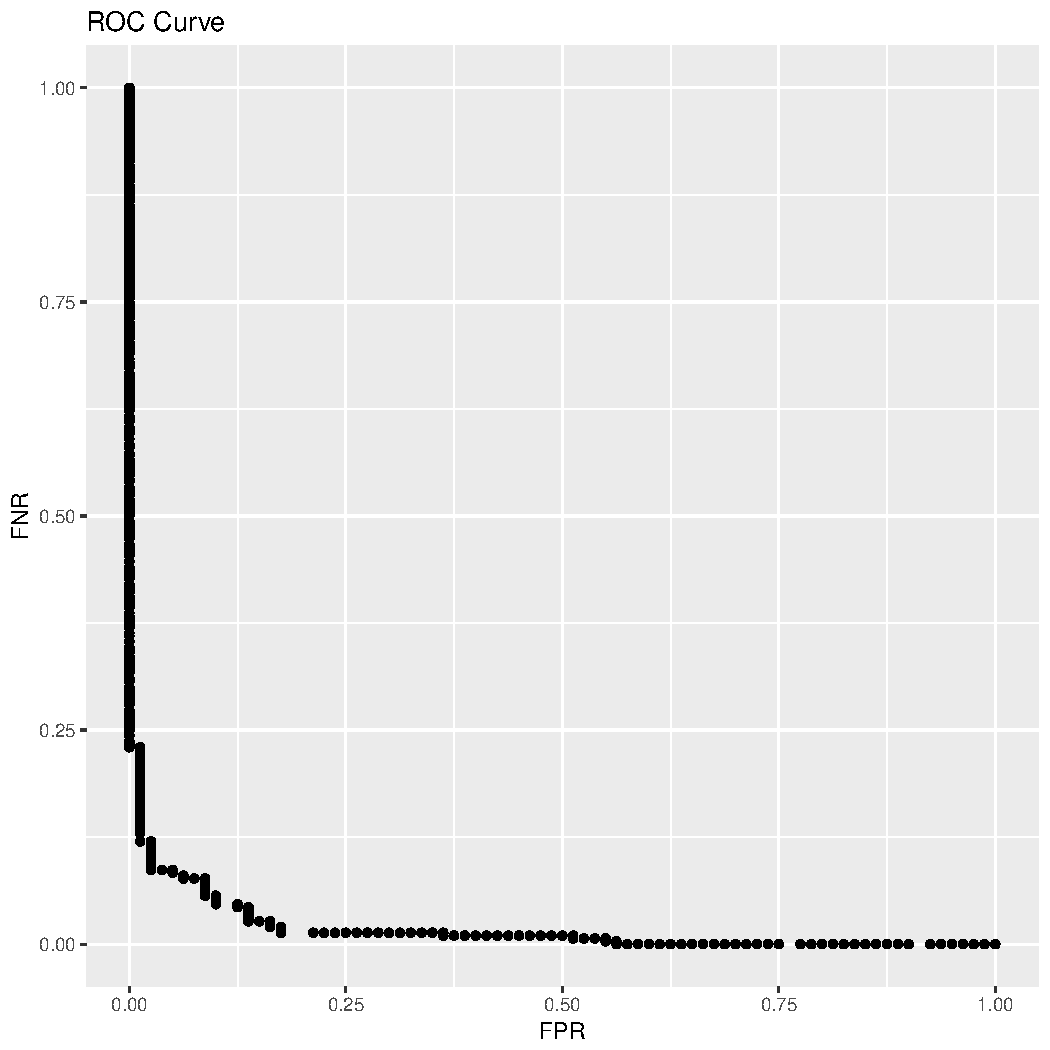
\includegraphics[keepaspectratio=true,width=0.45\textwidth]{authentication_accuracy_vs_total_interactions.pdf}
\label{figure_authentication_accuracy}
\end{center}
\end{figure}

\begin{figure}[hbt]
\caption{}
\begin{center}
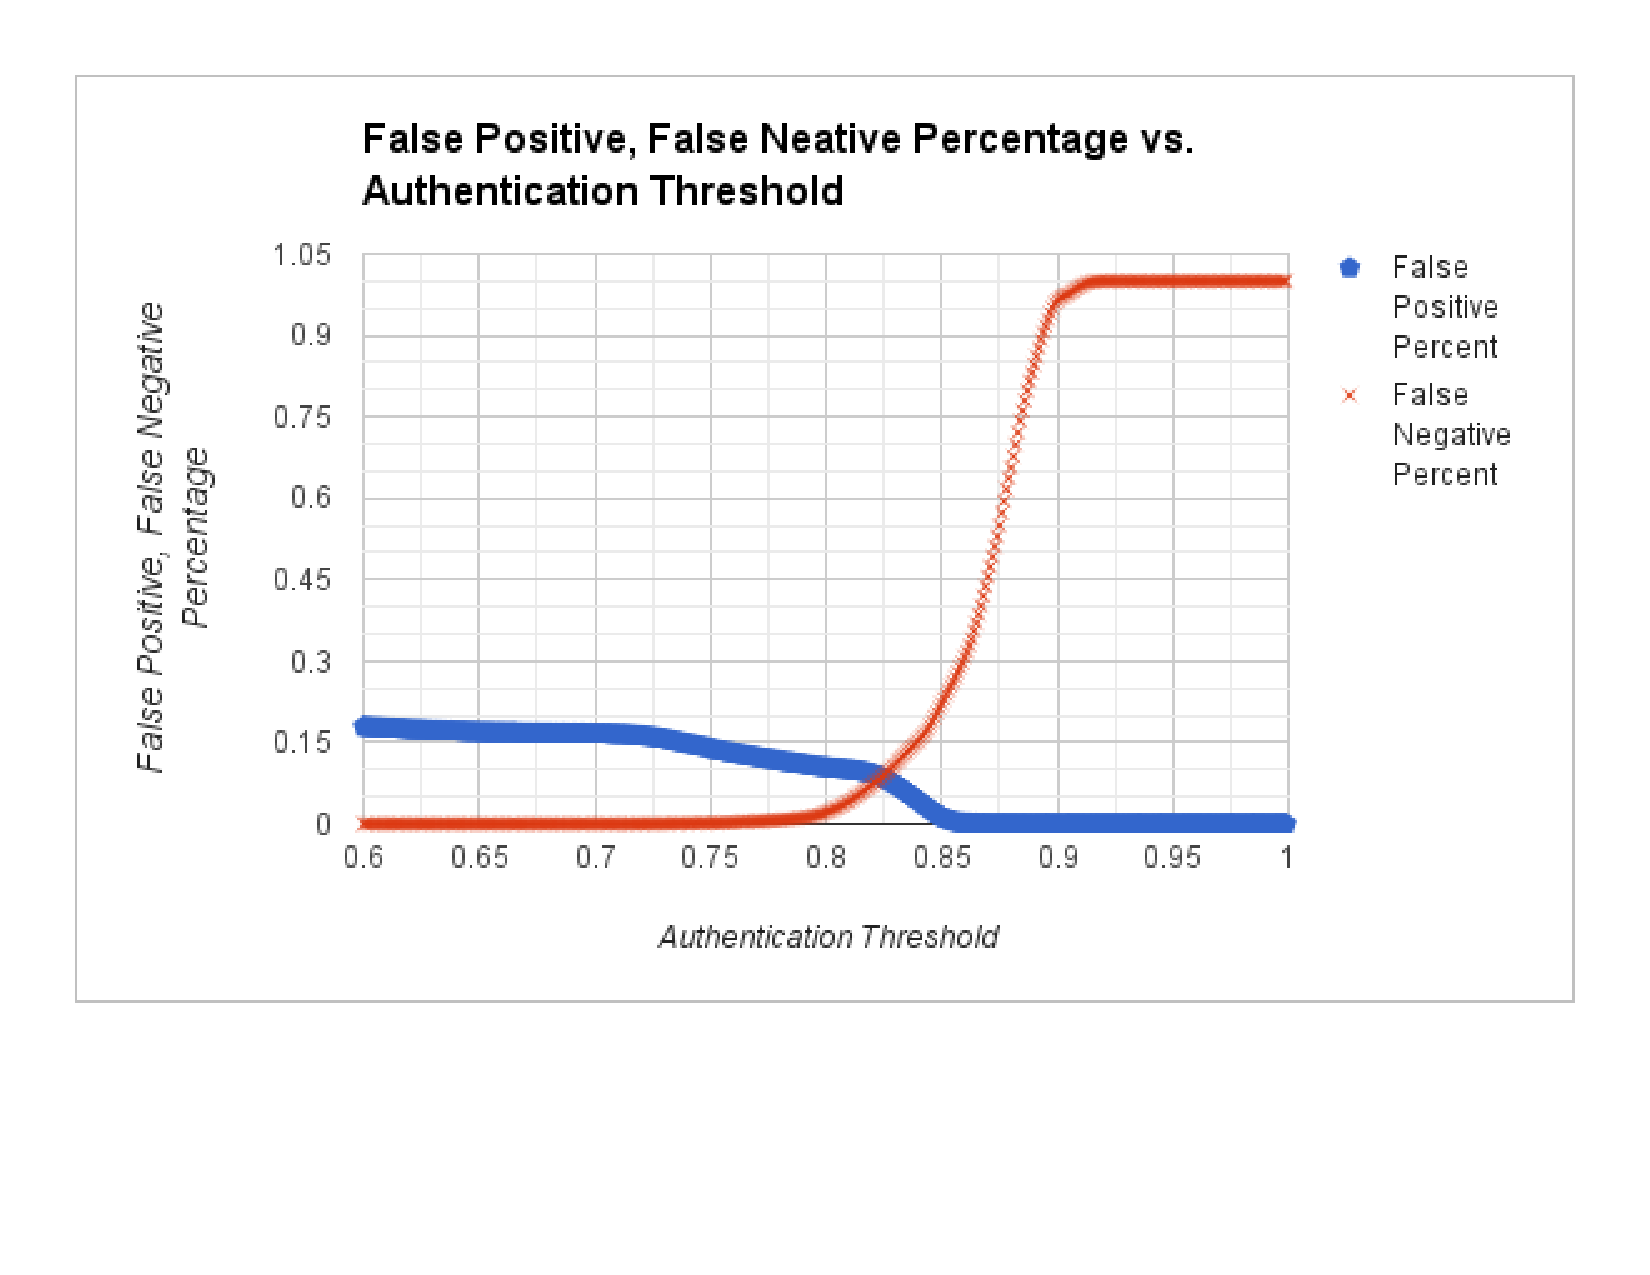
\includegraphics[keepaspectratio=true,width=0.45\textwidth]{false_positive_vs_authentication_threshold.pdf}
\label{figure_false_positive}
\end{center}
\end{figure}

\begin{figure}[hbt]
\caption{}
\begin{center}
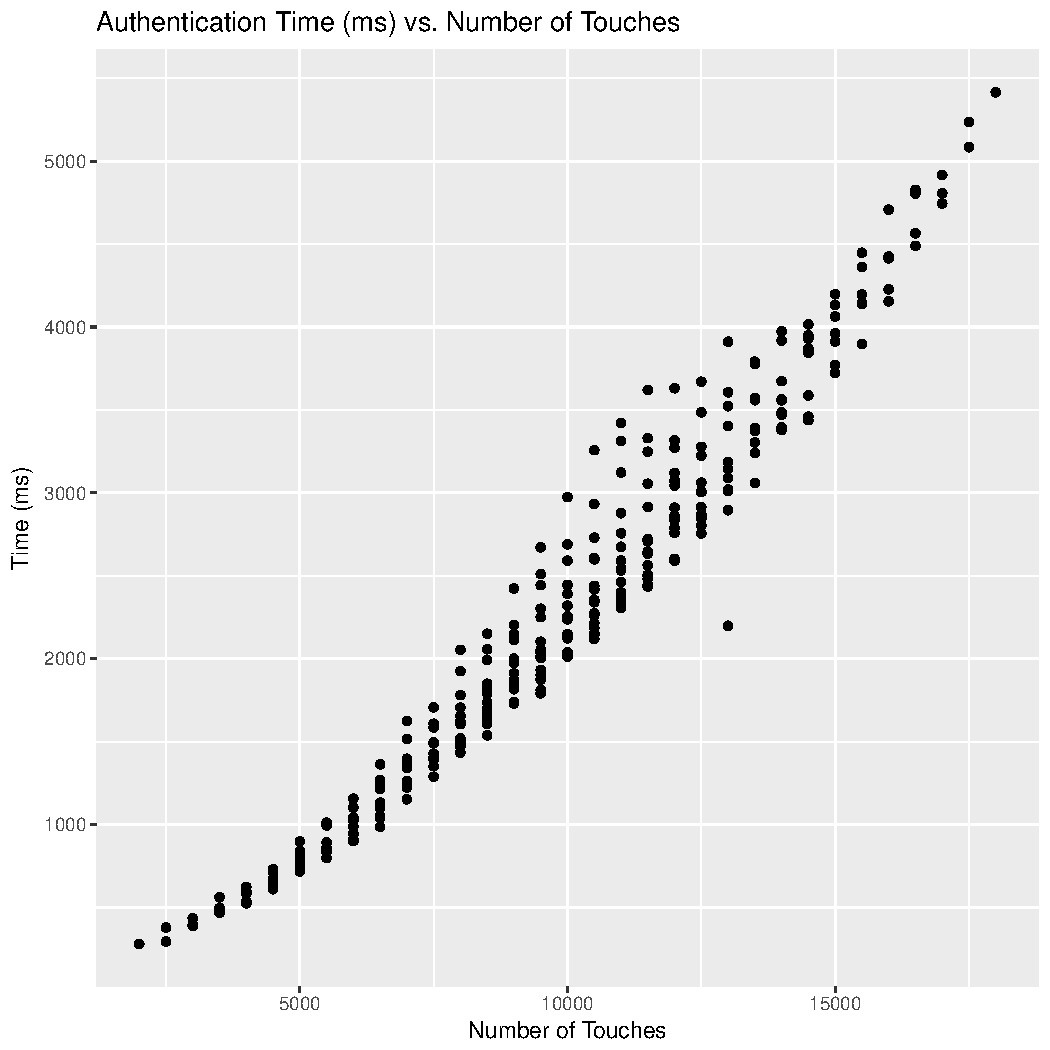
\includegraphics[keepaspectratio=true,width=0.45\textwidth]{nexus_7_runtimes.pdf}
\label{figure_nexus_7_runtimes}
\end{center}
\end{figure}

\lipsum[0-8]

% include mention of some problems which presented themselves
Some notable problems presented themselves
throughout the course of this work
which could influence the usability of such a 
system in a practical sense.
%
The Android \textbf{MotionEvent} class \textbf{getPressure()} method
used to collect pressure data in our system
does not always return a high granularity of values.
The pressure values are sometimes grouped
into large steps.
There might, for example,
be $8$ steps between $0.0$ and $1.0$ on some devices.
This is a problem for our system which uses
these pressure values to understand user variability.
%
The problem seems to be device dependent
suggesting that the device drivers may have a role to play
in decreasing the reported graininess of pressure.
Another possibility might be the values
reported by the sensors,
Perhaps these sensors only report a small number of steps.
%TODO state the performance impact on our system

% tie all analysis's back to the claims
%TODO